\documentclass[10pt,a4paper,twocolumn]{article}

\usepackage[T1]{fontenc}
\usepackage[utf8]{inputenc}
\usepackage[brazil]{babel}
\usepackage{lmodern}
\usepackage{microtype}
\usepackage[a4paper,top=1.7cm,bottom=1.9cm,left=1.7cm,right=1.7cm]{geometry}
\usepackage{amsmath}
\usepackage{graphicx}
\usepackage{booktabs}
\usepackage[font=small,labelfont=bf,skip=4pt]{caption}
\usepackage[compact]{titlesec}
\usepackage{enumitem}
\usepackage[round,semicolon]{natbib}
\usepackage{xurl}
\usepackage[hidelinks]{hyperref}

\setlength{\columnsep}{0.6cm}
\titleformat{\section}{\normalfont\large\bfseries}{\thesection}{0.6em}{}
\titlespacing*{\section}{0pt}{1.1ex plus .3ex}{0.6ex}
\setlist{nosep,leftmargin=1.2em}
\newcommand{\var}[1]{\texttt{#1}}
\renewcommand{\bibname}{Referências}
\renewcommand{\refname}{Referências}

\title{\vspace{-1.2cm}\textbf{Redes bayesianas aplicadas às colisões entre fauna e aeronaves}\\[2pt]
\large Trabalho Prático 3 -- Fundamentos de Inteligência Artificial}
\author{Arthur Fernandes (2020026800) \quad Bruno Lima Soares (2022055785)\\ Eduarda Amaral (matrícula a preencher)\\[2pt]
\small Departamento de Engenharia Elétrica -- Professores João Pedro Campos e Cristiano Leite de Castro}
\date{\small Belo Horizonte, novembro de 2026}

\begin{document}
\maketitle

\section{Introdução}

Colisões entre aeronaves e animais são frequentes. Só entre 2017 e 2025, a agência de aviação civil dos Estados Unidos
(FAA) recebeu mais de 159 mil relatos. Quase todos terminam sem consequência, mas alguns danificam a aeronave e obrigam o
piloto a abortar uma decolagem ou a pousar antes do previsto. Neste trabalho, usamos a base pública da FAA
\citep{faa2026} para construir uma rede bayesiana que relaciona o contexto do voo, a aeronave e o animal atingido com o
dano e com o efeito no voo.

Uma rede bayesiana representa as variáveis como nós de um grafo acíclico dirigido (DAG) e escreve a distribuição
conjunta como um produto de distribuições condicionais, uma por nó, cada uma condicionada aos pais do nó no grafo
\citep{koller2009}:
\begin{equation}
P(X_1,\dots,X_n)=\prod_{i=1}^{n} P\big(X_i \mid \mathrm{Pa}(X_i)\big).
\label{eq:fatoracao}
\end{equation}
A estrutura define quais variáveis influenciam quais, e as tabelas de probabilidade condicional (CPTs) dizem quanto.
Com o modelo pronto, é possível calcular a probabilidade de qualquer variável dada qualquer combinação de evidências,
e o próprio grafo ajuda a explicar as respostas. Formulamos quatro perguntas para a rede responder:
\begin{enumerate}[label=\textbf{Q\arabic*.}]
\item dado o perfil de uma colisão (aeronave, motor, animal e fase do voo), qual a probabilidade de dano?
\item quando o motor ingere um animal, qual a chance de isso afetar o voo?
\item se o motor teve de ser desligado, o que provavelmente atingiu a aeronave?
\item se o manejo de fauna nos aeroportos afastasse os animais médios e grandes, quanto cairia o risco de dano?
\end{enumerate}

\section{Dados e pré-processamento}

A planilha da FAA tem 360.384 relatos, enviados por pilotos, aeroportos, companhias aéreas e equipes de manutenção.
Ficamos com os anos de 2017 a 2025 (159.245 relatos): o critério de dano está estável desde 2017, e 2026 ainda está
incompleto. Removemos os 65.745 relatos sem nível de dano, que é o nosso alvo, e os 20.623 sem fase do voo, que
quase sempre são carcaças encontradas na pista, sem nenhuma informação sobre o voo. Também saíram 65 relatos sem a
quantidade de animais atingidos. Sobraram 72.812 colisões, das quais 5.608 (7,7\%) tiveram dano.

A rede tem as 14 variáveis categóricas da Tabela~\ref{tab:variaveis}. Nas variáveis que não são o alvo, preferimos
transformar o valor faltante num estado próprio, \var{desconhecido}, a descartar a linha: só a variável \var{avisado}
falta em metade dos relatos. A única variável contínua, a altura, foi discretizada em três faixas pelos tercis dos
valores positivos, que ficaram em 1 a 350, 350 a 1.700 e 1.700 a 32.000 pés. Altura zero virou o estado \var{solo}
(31\% das colisões), e o vazio virou \var{desconhecido}. As demais categorias foram agrupadas por regras de texto e
renomeadas em português; na quantidade atingida, juntamos ``2 a 10'' e ``mais de 10'', porque só 347 colisões tinham
mais de 10 animais. O nível de dano (nenhum, leve ou grave) ficou fora da rede, porque define \var{houve\_dano} por
completo e criaria uma dependência sem informação nova.

\begin{table}[t]
\centering\small
\caption{Variáveis da rede e seus estados. Nas variáveis com \% desc.\ positivo, há também o estado
\var{desconhecido}.}
\label{tab:variaveis}
\setlength{\tabcolsep}{3pt}
\begin{tabular}{@{}lp{4.55cm}r@{}}
\toprule
Variável & Estados & \% desc. \\
\midrule
\var{estacao} & inverno, primavera, verão, outono & 0,0 \\
\var{periodo} & amanhecer, dia, anoitecer, noite & 7,4 \\
\var{fase\_voo} & solo/táxi, corrida de decolagem, subida, rota, aproximação, corrida de pouso & 0,0 \\
\var{altura} & solo, baixa, média, alta (tercis) & 22,3 \\
\var{ceu} & sem nuvens, algumas nuvens, encoberto & 23,2 \\
\var{massa\_aeronave} & leve, média, pesada & 0,6 \\
\var{motor} & pistão, turboélice, jato, helicóptero & 0,8 \\
\var{animal} & ave, morcego, terrestre & 0,0 \\
\var{tamanho\_animal} & pequeno, médio, grande & 24,2 \\
\var{qtd\_atingida} & um, dois ou mais & 0,0 \\
\var{avisado} & sim, não (aviso de fauna ao piloto) & 50,7 \\
\var{ingestao\_motor} & não, sim & 0,0 \\
\var{houve\_dano} & não, sim (alvo principal) & 0,0 \\
\var{efeito\_voo} & nenhum, pouso de precaução, decolagem abortada, desligamento do motor, outro & 0,0 \\
\bottomrule
\end{tabular}
\end{table}

Uma primeira olhada nas taxas de dano já mostra onde está a informação. Animal grande causa dano em 44,0\% das
colisões, e animal pequeno, em 2,9\%. Aeronaves leves sofrem dano em 19,7\% dos casos, contra 4,9\% das pesadas, e a
ingestão pelo motor leva a taxa de 7,1\% para 25,1\%. Período do dia e condição do céu quase não mudam nada (todas as
taxas entre 6,7\% e 9,3\%), com exceção da estação: no inverno a taxa chega a 13,9\%, e no verão fica em 5,2\%.

\section{Métodos}

\textbf{Aprendizado de estrutura.} Usamos dois métodos citados no material da disciplina
\citep{campos2025}. O primeiro é o Hill-Climbing com o score BIC \citep{schwarz1978},
\begin{equation}
\mathrm{BIC}(G)=\log P(D\mid\hat\theta_G)-\frac{k_G}{2}\log n,
\end{equation}
em que o primeiro termo é a log-verossimilhança dos $n$ registros com os parâmetros de máxima verossimilhança e o
segundo penaliza os $k_G$ parâmetros livres do grafo. O algoritmo começa do grafo vazio e, a cada passo, aplica a
inclusão, remoção ou inversão de aresta que mais aumenta o score, até nenhuma operação melhorar. O resultado é um ótimo
local. Rodamos duas versões. Na versão livre, qualquer direção é permitida. Na versão por camadas, as variáveis são
divididas em grupos na ordem dos acontecimentos (contexto; aeronave e voo; animal; ingestão; dano; efeito no voo), e
nenhuma seta pode voltar para um grupo anterior. A segunda versão existe porque as intervenções da Q4 e da
Seção~\ref{sec:explicacao} dependem da direção das setas.

O segundo método é o de Chow-Liu \citep{chow1968}. Ele calcula a informação mútua entre cada par de variáveis e
monta a árvore que liga todas elas com a maior soma de informação mútua; depois, orienta as arestas a partir de uma
raiz. Como numa árvore nenhum nó tem dois pais, todas as orientações são equivalentes e têm o mesmo BIC.

Para comparar estruturas, lembramos que grafos diferentes podem ser equivalentes, isto é, representar as mesmas
independências condicionais e ter o mesmo BIC. Só as arestas forçadas por v-estruturas ($A\to B\leftarrow C$) têm a
direção determinada pelos dados \citep{koller2009}. Por isso, além de comparar as arestas uma a uma, comparamos as
classes de equivalência com a distância de Hamming estrutural (SHD).

\textbf{Parâmetros e inferência.} A estimação por máxima verossimilhança usa a frequência de cada estado em cada
combinação dos pais. A estimação bayesiana com prior BDeu \citep{heckerman1995} soma pseudo-contagens antes de
normalizar,
\begin{equation}
\hat\theta_{ijk}=\frac{N_{ijk}+\alpha/(q_i r_i)}{N_{ij}+\alpha/q_i},
\end{equation}
em que $r_i$ é o número de estados do nó, $q_i$ o de combinações dos pais e $\alpha$ o tamanho amostral equivalente.
Escolhemos o estimador e o valor de $\alpha$ pela log-verossimilhança média num conjunto de teste com 20\% dos dados.
As consultas usam eliminação de variáveis, que é exata. Para as intervenções, usamos o operador $\mathrm{do}(X=x)$
\citep{pearl2009}: cortam-se as arestas que chegam em $X$, fixa-se o seu valor e calcula-se a consulta no grafo
modificado. Tudo foi feito com o pgmpy 1.1.2 \citep{ankan2015}, num notebook que baixa os dados e reproduz cada número
deste relatório.

\section{Estrutura elicitada e estruturas aprendidas}

Antes de rodar qualquer algoritmo, desenhamos a rede que achávamos fazer sentido, com 17 arestas
(Figura~\ref{fig:comparacao}, no alto à esquerda). A ideia era que o contexto do voo influencia qual animal está no
caminho (estação e período mudam a fauna presente; a fase do voo define a altura, e a altura limita o tipo de animal),
que o animal e a aeronave determinam a ingestão e o dano (o tamanho define a energia do impacto, aeronaves leves são
menos resistentes, turbofans aspiram o ar à frente), e que o dano e a ingestão determinam o efeito no voo.

\begin{figure*}[t]
\centering
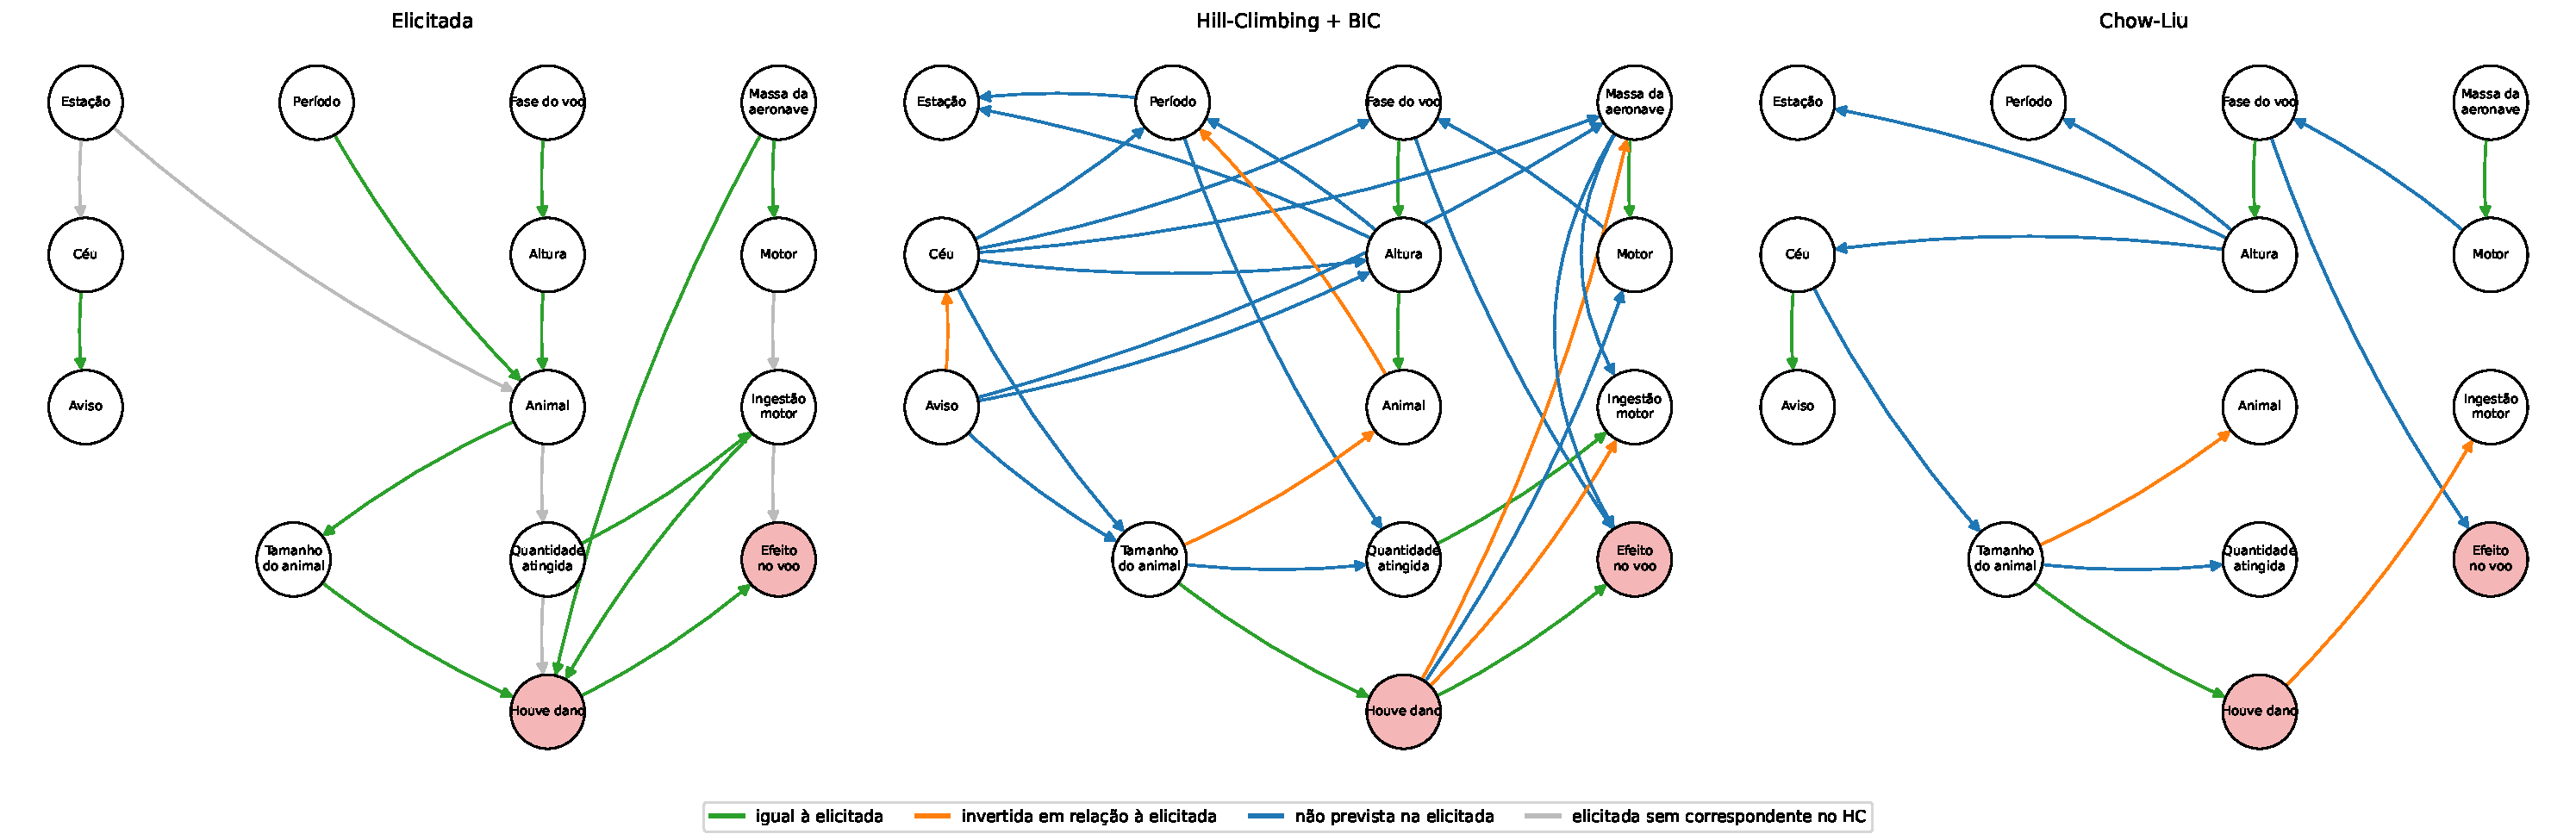
\includegraphics[width=0.84\textwidth]{figuras/fig_comparacao.pdf}
\caption{Rede elicitada (no alto, à esquerda) e as três redes aprendidas. Verde: aresta igual à elicitada; laranja:
invertida; azul: não prevista no desenho; cinza (só na elicitada): aresta que não aparece no Hill-Climbing por
camadas. Os nós em vermelho são os alvos.}
\label{fig:comparacao}
\end{figure*}

\begin{table}[t]
\centering\small
\caption{Comparação das estruturas. O SHD é calculado entre as classes de equivalência.}
\label{tab:estruturas}
\setlength{\tabcolsep}{2.6pt}
\begin{tabular}{@{}lrrrrr@{}}
\toprule
Estrutura & Arestas & Parâm. & BIC & \multicolumn{2}{c}{SHD vs} \\
\cmidrule(l){5-6}
 & & & & elicit. & livre \\
\midrule
Elicitada & 17 & 377 & $-736.569$ & 0 & 28 \\
HC livre & 31 & 1.302 & $-696.115$ & 28 & 0 \\
HC por camadas & 31 & 1.345 & $-697.125$ & 25 & 13 \\
Chow-Liu & 13 & 180 & $-709.954$ & 21 & 25 \\
\bottomrule
\end{tabular}
\end{table}

A Tabela~\ref{tab:estruturas} mostra que o nosso desenho ficou bem atrás. Até a árvore de Chow-Liu, com apenas 13
arestas, tem BIC 26 mil pontos melhor. Ficaram de fora dependências fortes, como \var{motor}--\var{fase\_voo},
\var{altura}--\var{periodo} e \var{ceu}--\var{tamanho\_animal}, e as 13 arestas da árvore aparecem, com alguma
orientação, nas duas versões do Hill-Climbing.

Na rede por camadas, nove das 17 arestas desenhadas aparecem exatamente como previmos, entre elas
$\var{tamanho\_animal}\to\var{houve\_dano}$, $\var{massa\_aeronave}\to\var{houve\_dano}$,
$\var{ingestao\_motor}\to\var{houve\_dano}$ e $\var{houve\_dano}\to\var{efeito\_voo}$. O Hill-Climbing livre acerta
oito, mas coloca o dano como pai da ingestão e da quantidade de animais atingidos, e essas duas direções são forçadas por
v-estruturas. Isso não tem sentido físico, mas o BIC não procura causas, e sim a forma mais compacta de escrever a
distribuição conjunta. Exigir a ordem por camadas custou 1.010 pontos de BIC, cerca de 0,15\% do score, e foi a rede
por camadas que usamos daí em diante.

As cinco arestas desenhadas que a rede por camadas não aceitou têm informação mútua muito baixa,
entre 0,0009 e 0,0027 nats. O caso mais interessante é $\var{ingestao\_motor}\to\var{efeito\_voo}$. Incluí-la aumenta a
log-verossimilhança em 156, mas cria 192 parâmetros, e cada parâmetro custa $\tfrac{1}{2}\log n\approx 5{,}6$ pontos; o
BIC piora 919. Como só 3\% das colisões têm ingestão, um efeito grande nesses casos pesa pouco na base inteira.

Entre as 19 arestas que só a rede por camadas tem, nove ligam variáveis com muitos \var{desconhecido} (aviso, céu,
altura, período, estação e tamanho). Quem deixa um campo do relato em branco costuma deixar outros: quando o céu é
desconhecido, o período também é desconhecido com frequência 2,5 vezes maior que a média. Como o faltante virou um
estado, a rede aprende esse padrão de preenchimento, que não diz nada sobre o fenômeno. Outras arestas novas são
legítimas e simplesmente não tínhamos pensado nelas, como $\var{fase\_voo}\to\var{efeito\_voo}$: as 800 decolagens
abortadas aconteceram, como era de se esperar, na corrida de decolagem.

\section{Parâmetros e inferência}

A máxima verossimilhança deu probabilidade zero a 15 colisões do conjunto de teste, com combinações de pais que não
apareceram no treino. Com o prior BDeu isso não acontece, e os valores de $\alpha$ entre 1 e 100 ficaram muito
próximos; usamos $\alpha=50$, o melhor deles. Na rede final, \var{houve\_dano} tem três pais (ingestão, massa da
aeronave e tamanho do animal) e um filho, o efeito no voo. A CPT do dano vai de 1,9\% (animal pequeno, sem ingestão,
aeronave pesada) a 91,8\% (animal grande, com ingestão, aeronave leve). A Tabela~\ref{tab:consultas} resume as
respostas.

\begin{table}[t]
\centering\small
\caption{Respostas da rede por camadas e frequências observadas nos $n$ registros com a mesma evidência, em \%. Na Q2 e na
Q3, a linha ``variante'' é a rede com a aresta $\var{ingestao\_motor}\to\var{efeito\_voo}$ obrigatória.}
\label{tab:consultas}
\footnotesize
\setlength{\tabcolsep}{2.5pt}
\begin{tabular}{@{}lrrr@{}}
\toprule
Consulta & Rede & Dados & $n$ \\
\midrule
\multicolumn{4}{@{}l}{\textit{Q1: P(dano $\mid$ perfil)}} \\
\quad jato pesado, ave pequena, aproximação & 2,2 & 2,1 & 15.548 \\
\quad animal grande & 39,2 & 44,0 & 4.259 \\
\quad leve, pistão, animal terrestre & 59,5 & 69,4 & 235 \\
\quad leve, pistão, animal grande, rota & 62,3 & 81,7 & 115 \\
\multicolumn{4}{@{}l}{\textit{Q2: P(algum efeito no voo $\mid$ ingestão)}} \\
\quad rede por camadas & 6,5 & 15,1 & 2.240 \\
\quad variante & 14,4 & 15,1 & 2.240 \\
\multicolumn{4}{@{}l}{\textit{Q3: P(animal grande $\mid$ desligamento do motor)}} \\
\quad rede por camadas & 19,5 & 38,2 & 110 \\
\quad variante & 7,5 & 38,2 & 110 \\
\multicolumn{4}{@{}l}{\textit{Q4: probabilidade de dano}} \\
\quad sem evidência & 7,41 & 7,70 & 72.812 \\
\quad observando tamanho = pequeno & 3,04 & 2,93 & 42.317 \\
\quad $\mathrm{do}(\text{tamanho} = \text{pequeno})$ & 3,06 & -- & -- \\
\bottomrule
\end{tabular}
\end{table}

Na Q1, a rede acerta o perfil mais comum, mas subestima o risco quando o animal é grande. O motivo está na ligação
entre massa da aeronave e tamanho do animal. Nos dados, 31,6\% das colisões com animal grande envolvem aeronaves leves;
a rede, que liga essas variáveis só de forma indireta, estima 15,9\%, e como as leves sofrem mais dano, a estimativa
cai. O Hill-Climbing livre comete o mesmo erro (39,2\% para animal grande), então ele não vem da ordem por camadas.

A Q2 é onde a rede mais falha. Nos dados, a ingestão faz a chance de algum efeito no voo subir de 6,3\% para 15,1\%;
na rede, quase nada muda. Sem a aresta direta, a ingestão só chega ao efeito por dois caminhos que se anulam: pelo
dano ela aumenta o risco, mas também indica um jato pesado (88\% dos casos), e jatos pesados raramente registram efeito
no voo. Obrigar a aresta resolve a Q2, mas a busca, para não pagar parâmetros demais, troca
$\var{houve\_dano}\to\var{efeito\_voo}$ pela aresta nova, e a Q3 piora de 19,5\% para 7,5\%. O BIC e a
log-verossimilhança no teste também pioram ($-697.902$ contra $-697.125$; $-9{,}537$ contra $-9{,}527$ por registro).
Com tantos parâmetros em jogo, o nó do efeito no voo não comporta as duas setas ao mesmo tempo, e a melhor escolha
depende da pergunta. Mantivemos a rede sem a aresta, que é melhor pelos dois critérios.

Mesmo sem a variante, a Q3 só acerta a direção: o desligamento do motor leva a chance de animal grande de 5,5\% (quando não há
efeito no voo) para 19,5\%, contra 38,2\% nos dados. O efeito no voo só se liga ao animal através do dano, e a informação se dilui nesse
raciocínio em cadeia. Na Q4, a intervenção que representa um manejo de fauna perfeito, sem animais médios ou grandes,
reduz o risco de dano de 7,41\% para 3,06\%, menos da metade. Observar e intervir dão quase o mesmo valor porque os
pais do tamanho do animal (altura, céu e aviso) quase não afetam o dano por outros caminhos.

\section{Explicando uma predição}
\label{sec:explicacao}

Escolhemos primeiro a colisão com dano em que a rede tinha mais certeza, entre as que ocorreram na subida ou em rota,
com ingestão e sem nenhum estado desconhecido. É a colisão 1577229, de 2024: uma ave grande atingiu uma aeronave leve a
pistão durante a subida e entrou no motor. A rede dá 91,8\% de chance de dano, cerca de 12 vezes a média.

\begin{figure}[t]
\centering
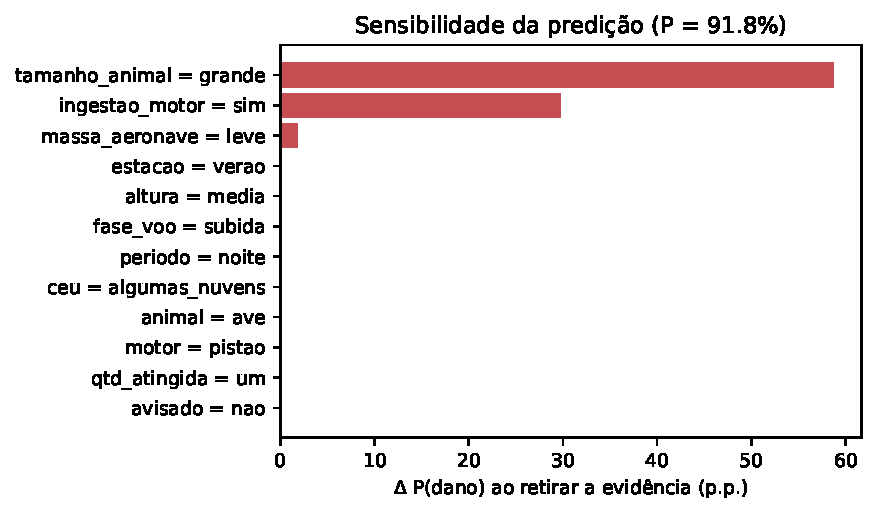
\includegraphics[width=\columnwidth]{figuras/fig_tornado.pdf}
\caption{Quanto a probabilidade de dano da colisão 1577229 cai quando se retira cada evidência.}
\label{fig:tornado}
\end{figure}

A explicação começa pelo \emph{Markov blanket} do dano, formado por pais, filhos e outros pais dos filhos. Os três pais
estão na evidência, e o efeito no voo não foi observado; assim, a predição é simplesmente uma linha da CPT, e as outras
nove variáveis ficam d-separadas do alvo. A análise de sensibilidade da Figura~\ref{fig:tornado} retira uma evidência
de cada vez. Sem saber que a ave era grande, a estimativa cairia para 33,1\%, e sem saber da ingestão, para 62,1\%.
Retirar a massa quase não muda nada (90,0\%), porque o motor a pistão já indica uma aeronave leve, e a rede recupera a
informação pelas variáveis vizinhas. Nas intervenções, trocar a ave por uma pequena leva a 19,8\%, e impor que não
houve ingestão, a 62,0\%, com o mesmo valor observando ou intervindo, já que os pais de cada variável trocada estão na
evidência. Na rede livre isso não funcionava: lá a ingestão era filha do dano, e impor que ela não ocorreu não mudava
o risco. O notebook também gera uma explicação em linguagem natural com esses números.

O caso oposto rende mais. Entre as colisões com dano e sem estados desconhecidos, a de menor probabilidade prevista é
a 971157, de 2019: um jato pesado atingiu uma ave pequena na aproximação, à noite, sem ingestão, e a rede deu 1,9\%.
Houve dano leve, sem efeito no voo. A rede, porém, não estava descalibrada. Das 31.284 colisões com os mesmos valores
dos pais do dano, 1,9\% tiveram dano; entre as 202 com toda a evidência idêntica, foram 7. Nenhuma troca isolada
explicaria esse dano com folga: com uma ave grande, a estimativa iria a 30,7\%, e com ingestão, a 10,5\%. Saber que
não houve efeito no voo também não ajuda, porque é o que acontece na maioria das colisões. O que separa essas 7
colisões das outras não está na rede: a parte da aeronave atingida e a velocidade no impacto, que a FAA registra mas
que não usamos, ou a espécie exata, já que o tamanho é uma estimativa de quem relata.

\section{Limitações}

O tratamento dos faltantes como estado manteve a base inteira, mas trouxe para a rede dependências que vêm do jeito de
preencher o relato. O BIC descarta efeitos fortes que só aparecem em poucos casos, como o da ingestão sobre o efeito no
voo, e a solução para uma pergunta pode piorar outra. A ordem por camadas é uma hipótese nossa, e as intervenções só
valem dentro dela: a rede foi ajustada para descrever os dados, não para validar mecanismos. Também vimos que o
Hill-Climbing é sensível a empates. Como inverter uma aresta muitas vezes não muda o score, a rede livre mudava de uma
execução para outra até fixarmos a ordem de desempate no notebook.

\begin{thebibliography}{9}
\setlength{\itemsep}{1pt}
\small

\bibitem[{Ankan; Panda}(2015)]{ankan2015}
ANKAN, A.; PANDA, A. pgmpy: probabilistic graphical models using Python. \emph{In}: PYTHON IN SCIENCE CONFERENCE, 14.,
2015, Austin. \textbf{Proceedings} [...]. Austin: SciPy, 2015. p.~6--11.

\bibitem[{Campos; Castro}(2025)]{campos2025}
CAMPOS, J. P.; CASTRO, C. L. de. \textbf{Aprendizado estrutural de redes bayesianas}. Belo Horizonte: Departamento
de Engenharia Elétrica, 2025. 62 slides. Notas de aula da disciplina Fundamentos de Inteligência Artificial.

\bibitem[{Chow; Liu}(1968)]{chow1968}
CHOW, C. K.; LIU, C. N. Approximating discrete probability distributions with dependence trees. \textbf{IEEE
Transactions on Information Theory}, v.~14, n.~3, p.~462--467, 1968.

\bibitem[{Federal Aviation Administration}(2026)]{faa2026}
FEDERAL AVIATION ADMINISTRATION. \textbf{FAA Wildlife Strike Database}. Washington, DC: FAA, 2026. Disponível em:
\url{https://wildlife.faa.gov}. Acesso em: 14 nov. 2026.

\bibitem[{Heckerman; Geiger; Chickering}(1995)]{heckerman1995}
HECKERMAN, D.; GEIGER, D.; CHICKERING, D. M. Learning Bayesian networks: the combination of knowledge and statistical
data. \textbf{Machine Learning}, v.~20, n.~3, p.~197--243, 1995.

\bibitem[{Koller; Friedman}(2009)]{koller2009}
KOLLER, D.; FRIEDMAN, N. \textbf{Probabilistic graphical models}: principles and techniques. Cambridge, MA: MIT
Press, 2009.

\bibitem[{Pearl}(2009)]{pearl2009}
PEARL, J. \textbf{Causality}: models, reasoning, and inference. 2.~ed. Cambridge: Cambridge University Press, 2009.

\bibitem[{Schwarz}(1978)]{schwarz1978}
SCHWARZ, G. Estimating the dimension of a model. \textbf{The Annals of Statistics}, v.~6, n.~2, p.~461--464, 1978.

\end{thebibliography}

\end{document}
